\section{Architecture} \label{sec:Architecture}
Central to Bitcoin's architecture is a public ledger called the \emph{blockchain}, which stores all processed \emph{transactions} in chronological order. Transactions are processed by a loosely-organized network of \emph{miners} in a process called \emph{mining} (see Sect. \ref{sec:Mining}). In it the miner creates a \emph{block} with a set of unprocessed transactions and attempts to solve a \emph{proof-of-work puzzle} (see Sect. \ref{sec:ProofOfWork}). Once a valid solution has been found, the block including the solution is published throughout the network and accepted into the blockchain. In this section the structure of blocks and transactions will be discussed in detail. Note that the following description is based on the Bitcoin source code \cite{BitcoinSourceCode} and the Bitcoin Protocol Specification on Wikipedia \cite{Wikipedia_ProtocolSpec}. Furthermore, all data types denoted in the diagrams are explained in detail in \ref{sec:DataTypes}.

\subsection{Blocks} \label{sec:Blocks}
Each block is composed of a header and a payload. The header stores the current block header version (\textit{nVersion}), a reference to the previous block (\textit{HashPrevBlock}), the root node of the Merkle tree (\textit{HashMerkleRoot}), a timestamp (\textit{nTime}), a target value  (\textit{nBits}) and a nonce (\textit{nNonce}). Finally, the payload stores the number of transactions (\textit{\#vtx}) and the vector of transactions (\textit{vtx}) included in the block.

\begin{table}[ht!]
	\begin{tabularx}{\textwidth}{ | m{70pt} | >{\centering} m{60pt} | X |}

		\hline
		\textbf{Field name} &
		\bigcell{c}{\textbf{Type} \\ \textbf{(Size)}} &
		\textbf{Description}\\ \hline\hline
    
		nVersion &
		\bigcell{c}{int \\ (4 bytes)} &
		Block format version (currently 2). \\ \hline
		
		HashPrevBlock &
		\bigcell{c}{uint256 \\ (32 bytes)} &
		Hash of previous block header \newline
		$SHA256^{2}(nVersion || \dots || nNonce)$. \\ \hline
	
		HashMerkleRoot &
		\bigcell{c}{uint256 \\ (32 bytes)} &
		Top hash of the Merkle tree built from all transactions. \\ \hline
		
		nTime &
		\bigcell{c}{unsigned int \\ (4 bytes)} &
		Timestamp in UNIX-format of approximate block creation time. \\ \hline
	
		nBits &
		\bigcell{c}{unsigned int \\ (4 bytes)} &
		Target T for the proof-of-work problem in compact format. Full target value is derived as:\newline$T = 0xh_{2}h_{3}h_{4}h_{5}h_{6}h_{7} * 2^{8*(0xh_{0}h_{1} - 3)}$\\ \hline
	
		nNonce &
		\bigcell{c}{unsigned int \\ (4 bytes)} &
		Nonce allowing variations for solving the proof-of-work problem.\\ \hline
	
		\#vtx &
		\bigcell{c}{VarInt \\ (1-9 bytes)} &
		Number of transaction entries in \textit{vtx}. \\ \hline
	
		vtx[\,] &
		\bigcell{c}{Transaction \\ (Variable)} &
		Vector of transactions. \\ \hline
	\end{tabularx}
	\vspace{5pt}
	\caption{Block Structure Description}
	\label{table:CBlock}
\end{table}

\vspace{-30pt}
\clearpage

\subsubsection*{nVersion}
The version field stores the version number of the block format. Ever since BIP0034 \cite{BIP0034} is in place, the block format version is 2 and blocks of any other version are neither relayed nor mined.

\subsubsection*{HashPrevBlock}
This field stores the reference to the previous block, computed as a hash over the block header as depicted in Fig. \ref{fig:HashPrevBlock}.
\begin{figure}[ht!]
 \centering
 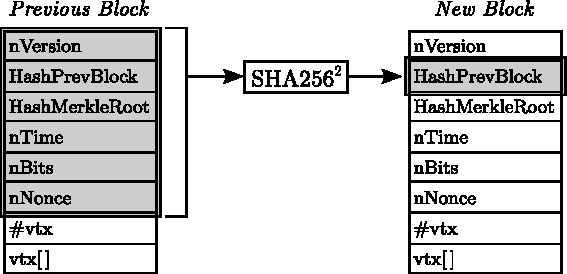
\includegraphics[scale=0.9]{images/HashPrevBlock.pdf}
 \caption{Block Reference Computation} \label{fig:HashPrevBlock}
\end{figure}

\noindent
A double-SHA256 hash is calculated over the concatenation of all elements in the previous block header:
\begin{equation}
\begin{aligned}
SHA256^{2}(nVersion||HashPrevBlock||HashMerkleRoot||nTime||nBits||nNonce)
\label{eqn:HashPrevBlock}
\end{aligned}
\end{equation}

\noindent
The reference functions as a chaining link in the blockchain. By including a reference to the previous block, a chronological order on blocks, and thus transactions as well, is imposed.


\subsubsection*{HashMerkleRoot}
This field stores the root of the Merkle hash tree. It is used to provide integrity of all transactions included in the block and is computed according to the scheme described in Sect. \ref{sec:MerkleTrees}. The parameters used for computing the tree are double-SHA256 as the hashing algorithm and raw transactions as data blocks (see Table \ref{tab:TransactionRegular} and \ref{tab:TransactionCoinbase}).


\subsubsection*{nTime}
The time field stores the timestamp in UNIX format denoting the approximate block creation time. As the timestamp is a parameter included in block mining, it is fixed at the beginning of the process.


\subsubsection*{nBits}
The \textit{nBits} field stores a compact representation of a target value \emph{T}, which is utilized in the proof-of-work puzzle (see Sect. \ref{sec:Mining}). The target value is a 256 bit long number, whereas its corresponding compact representation is only 32 bits long and thus encoded with only 8 hex digits. The target value can be derived from its compact hexadecimal representation $\mathit{0xh_{0}h_{1}h_{2}h_{3}h_{4}h_{5}h_{6}h_{7}}$ with the formula
\begin{equation}
0xh_{2}h_{3}h_{4}h_{5}h_{6}h_{7} * 2^{8*(0xh_{0}h_{1} - 3)}
\end{equation}


\noindent
The upper bound for the target is defined as $\texttt{0x1D00FFFF}$ whereas there is no lower bound. The very first block, the genesis block, has been mined using the maximum target. In order to ensure that blocks are mined at a constant rate of one block per 10 minutes throughout the network, the target \emph{T} is recalculated every 2016 blocks based on the time $\mathit{t_{sum}}$ it took to mine, due to an off-by-one error \cite{nBitsCalc}, the last 2015 blocks:
\begin{equation}
T' = \dfrac{t_{sum}}{14*24*60*60s}*T
\end{equation}

\noindent
Note that $\mathit{t_{sum}}$ is calculated as the difference of the timestamps \textit{nTime} in the block header.

\subsubsection*{nNonce}
The nonce field contains arbitrary data and is used as a source of randomness for solving the proof-of-work problem. However, since it is fairly small in size with 4 bytes, it does not necessarily provide sufficient variation for finding a solution. Therefore, other sources exist and will be addressed in more detail in Sect. \ref{sec:Mining}.


\clearpage
\subsection{Transactions} \label{sec:Transactions}
In principle, there are two types of transactions - coinbase transactions and regular transactions. Coinbase transactions are special transactions in which new Bitcoins are introduced into the system. They are included in every block as the very first transaction and are meant as a reward for solving a proof-of-work puzzle. Regular transactions, on the other hand, are used to transfer existing Bitcoins amongst different users. From an architectural point of view, a coinbase transaction can be seen as a special case of a regular transaction. For this reason, the structure of a regular transaction will be discussed first, followed by the differences between coinbase and regular transactions.

\enlargethispage{2\baselineskip}
\subsection*{Regular transactions} \label{sec:RegularTransactions}
As mentioned in the previous section, each block in the blockchain includes a set of transactions. Every transaction consists of a transaction version (\textit{nVersion}), a vector of inputs (\textit{vin}) and a vector of outputs (\textit{vout}), both preceded by their count, and a transaction inclusion date (\textit{nLockTime}).
\begin{table}[ht!]
	\begin{tabularx}{\textwidth}{ | m{25pt} | m{70pt} | >{\centering} m{60pt} | X |} \hline
		\multicolumn{2}{|l|}{\textbf{Field name}} &
		\bigcell{c}{\textbf{Type} \\ \textbf{(Size)}} &
		\textbf{Description}\\ \hline\hline
    	
    	\multicolumn{2}{|l|}{nVersion} &
    	\bigcell{c}{int \\ (4 bytes)} &
    	Transaction format version (currently 1).\\ \hline
    	
	    \multicolumn{2}{|l|}{\#vin} &
	    \bigcell{c}{VarInt \\ (1-9 bytes)} &
    	Number of transaction input entries in \textit{vin}. \\ \hline
    	
		\multirow{9}{25pt}{\centering vin[\,]} &
		
		hash &
		\bigcell{c}{uint256 \\ (32 bytes)} &
		Double-SHA256 hash of a past transaction.\\ \cline{2-4}
		
		& n &
		\bigcell{c}{uint \\ (4 bytes)} &
		Index of a transaction output within the transaction specified by \textit{hash}. \\ \cline{2-4}

		& scriptSigLen &
		\bigcell{c}{VarInt \\ (1-9 bytes)} &
		Length of \textit{scriptSig} field in bytes. \\ \cline{2-4}
				
		& scriptSig &
		\bigcell{c}{CScript \\ (Variable)} &
		Script to satisfy spending condition of the transaction output (\textit{hash},\textit{n}). \\ \cline{2-4}
		
		& nSequence &
		\bigcell{c}{uint \\ (4 bytes)} &
		Transaction input sequence number. \\ \hline
    	
    	\multicolumn{2}{|l|}{\#vout} &
	    \bigcell{c}{VarInt \\ (1-9 bytes)} &
    	Number of transaction output entries in \textit{vout}. \\ \hline
    	
		\multirow{5}{25pt}{\centering vout[\,]} &
		
		nValue &
		\bigcell{c}{int64\_t \\ (8 bytes)} &
		Amount of $10^{-8}$ BTC. \\ \cline{2-4}
		
		& scriptPubkeyLen &
		\bigcell{c}{VarInt \\ (1-9 bytes)} &
		Length of \textit{scriptPubkey} field in bytes. \\ \cline{2-4}

		& scriptPubkey &
		\bigcell{c}{CScript \\ (Variable)} &
		Script specifying conditions under which the transaction output can be claimed. \\ \hline
    	
    	\multicolumn{2}{|l|}{nLockTime} &
    	\bigcell{c}{unsigned int \\ (4 bytes)} &
    	Timestamp past which transactions can be replaced before inclusion in block.\\ \hline
	
	\end{tabularx}
	\vspace{5pt}
	\caption{Regular Transaction Structure}
	\label{tab:TransactionRegular}
\end{table}

\subsubsection*{nVersion}
The version field stores the version number of the transaction format. The current transaction format version is 1.

\subsubsection*{\#vin}
This field stores the number of elements in the inputs vector \textit{vin}. It is encoded as a variable length integer (see \ref{sec:DataTypes}).

\subsubsection*{vin}
The \textit{vin} field stores a vector of one or more transaction inputs. Each transaction input is composed of a reference to a previous output (\textit{hash},\textit{n}), the length of the signature script field in bytes (\textit{scriptSigLen}),
the signature script field (\textit{scriptSig}) itself and a transaction sequence number (\textit{nSequence}).

\begin{itemize}
\item[-] (\textit{hash},\textit{n})~\\
A previous output is uniquely identified by the tuple (\textit{hash},\textit{n}). \textit{hash}, also referred to as the transaction ID (\textit{TxID}), is computed as a double-SHA256 hash of the raw transaction:
\begin{equation}
TxID = SHA256^{2}(Transaction)
\end{equation}

Hence, whilst a transaction is uniquely identified by its hash, the specific output within that transaction is identified by the output index \textit{n}. An example is given below in Fig. \ref{fig:PrevOut}.
\begin{figure}[ht!]
 \centering
 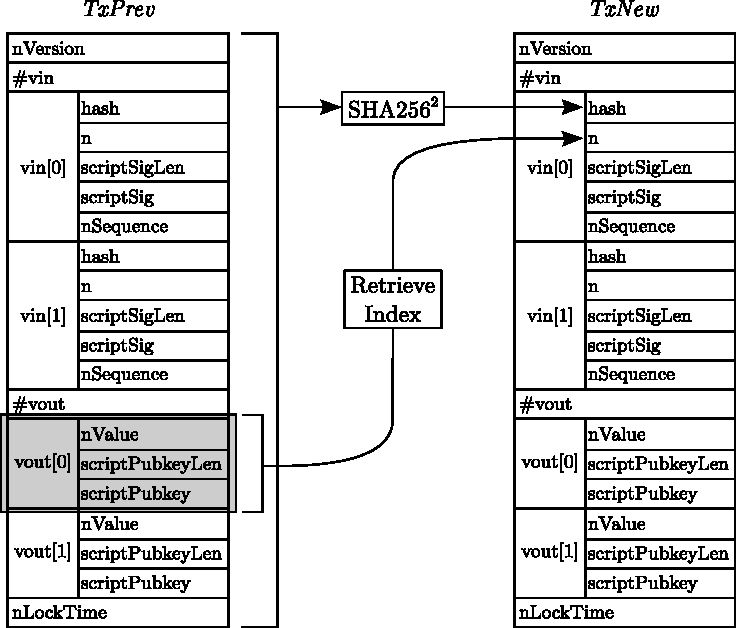
\includegraphics[scale=0.9]{images/Transaction2In2Out.pdf}
 \caption{Transaction Output Reference Computation} \label{fig:PrevOut}
\end{figure}

\item[-] \textit{scriptSigLen}~\\
This field stores the length of the signature script field \textit{scriptSig} in bytes. It is encoded as a variable length integer (see \ref{sec:DataTypes}).

\item[-] \textit{scriptSig}~\\
The signature script field contains a response script corresponding to the challenge script (see \textit{scriptPubey} field) of the referenced transaction output (\textit{hash},\textit{n}). More precisely, whilst the challenge script specifies conditions under which the transaction output can be claimed, the response script is used to prove that the transaction is allowed to claim it. More details on transaction verification can be found in Sect. \ref{sec:Script}.~\\

\item[-] \textit{nSequence}~\\
This field stores the transaction input sequence number. It was once intended for multiple signers to agree to update a transaction before including it in a block. If a signer was done updating, he marked his transaction input as final by setting the sequence number to the highest 4-byte integer value $\texttt{0xFFFFFFFF}$. More details can be found in Sect. \ref{sec:TransactionStandardness} under the Final Transaction Rule.
\end{itemize}

\subsubsection*{\#vout}
This field stores the number of elements in the output vector \textit{vout}. It is encoded as a variable length integer (see \ref{sec:DataTypes}).

\subsubsection*{vout}
The \textit{vout} field stores a vector of one or more transaction outputs. Each transaction output is composed of an amount of BTC being spent (\textit{nValue}), the length of the public key script (\textit{scriptPubkeyLen}) and the public key script (\textit{scriptPubkey}) itself.

\begin{itemize}
\item[-] \textit{nValue}~\\
The \textit{nValue} field stores the amount of BTC to be spent by the output. The amount is encoded in Satoshis, that is $10^{-8}$ BTC, allowing tiny fractions of a Bitcoin to be spent. However, note that in the reference implementation transactions with outputs less than a certain value are referred to as ``dust'' and are considered non-standard \cite{DustTransactions}. This value is currently by default 546 Satoshi and can be defined by each node manually. Dust transactions are neither relayed nor mined. More details on dust transactions can be found in \ref{sec:Calculations}.

\item[-] \textit{scriptPubkeyLen}~\\
This field stores the length of the public key script \textit{scriptPubkey} in bytes. It is encoded as a variable length integer (see \ref{sec:DataTypes}).

\item[-] \textit{scriptPubkey}~\\
The public key script field contains a challenge script for transaction verification. More precisely, whilst the challenge script specifies conditions under which the transaction output can be claimed, the response script (see \textit{scriptSig} field) is used to prove that the transaction is allowed to claim it. More details on transaction verification can be found in Sect. \ref{sec:Script}.

\end{itemize}

\subsubsection*{nLockTime}
This field stores the lock time of a transaction, i.e. a point in time past which the transaction should be included in a block. Once the lock time has been exceeded, the transaction is locked and can be included in a block. The lock time is encoded as either a timestamp in UNIX format or as a block number:
\begin{table}
\centering
	\begin{tabularx}{0.7\textwidth } {| >{\centering} m{40pt} | X |}
	\hline
	\textbf{Value} & \textbf{Description} \\ \hline\hline
	$0$ & Always locked. \\ \hline \rule{0pt}{10pt}
	$< 5*10^{8}$ & Block number at which transaction is locked. \\ \hline \rule{0pt}{10pt}
	$\geq 5*10^{8}$ & UNIX timestamp at which transaction is locked. \\ \hline
	\end{tabularx}
	\vspace{5pt}
	\caption{Lock Time Values}
	\label{tab:LockTime}
\end{table}
\vspace{-15pt}

\noindent
If all transaction inputs (see \textit{vin} field) have a final sequence number (see \mbox{\textit{nSequence}} field), then the lock time is ignored. More details can be found in Sect. \ref{sec:TransactionStandardness} under the Final Transaction Rule.


\clearpage
\subsection*{Coinbase Transactions} \label{sec:CoinbaseTransactions}
As can be seen in Table \ref{tab:TransactionCoinbase}, except for renaming the signature script field from \textit{scriptSig} to \textit{coinbase}, the data structure of the transaction remains the same. However, there are several constraints specific for a coinbase transaction. In the following the differences between a regular and a coinbase transaction will be explained.
\begin{table}[ht!]
	\begin{tabularx}{\textwidth}{ | m{30pt} | m{70pt} | >{\centering} m{60pt} | X |} \hline
		\multicolumn{2}{|l|}{\textbf{Field name}} &
		\bigcell{c}{\textbf{Type} \\ \textbf{(Size)}} &
		\textbf{Description}\\ \hline\hline
    	
    	\multicolumn{2}{|l|}{nVersion} &
    	\bigcell{c}{int \\ (4 bytes)} &
    	Transaction format version (currently 1).\\ \hline
    	
	    \multicolumn{2}{|l|}{\#vin} &
	    \bigcell{c}{VarInt \\ (1-9 bytes)} &
    	Number of transaction inputs entries in \textit{vin}. \\ \hline
    	
		\multirow{9}{30pt}{\centering vin[\,]} &
		
		hash &
		\bigcell{c}{uint256 \\ (32 bytes)} &
		Fixed double-SHA256 hash.\\ \cline{2-4}
		
		& n &
		\bigcell{c}{uint \\ (4 bytes)} &
		Fixed transaction output index. \\ \cline{2-4}

		& coinbaseLen &
		\bigcell{c}{VarInt \\ (1-9 bytes)} &
		Length of \textit{coinbase} field in bytes. \\ \cline{2-4}
				
		& coinbase &
		\bigcell{c}{CScript \\ (Variable)} &
		Encodes the block height and arbitrary data. \\ \cline{2-4}
		
		& nSequence &
		\bigcell{c}{uint \\ (4 bytes)} &
		Transaction input sequence number.\\ \hline
    	
    	\multicolumn{2}{|l|}{\#vout} &
	    \bigcell{c}{VarInt \\ (1-9 bytes)} &
    	Number of transaction output entries in \textit{vout}. \\ \hline
    	
		\multirow{5}{30pt}{\centering vout[\,]} &
		
		nValue &
		\bigcell{c}{int64\_t \\ (8 bytes)} &
		Amount of $10^{-8}$ BTC. \\ \cline{2-4}
		
		& scriptPubkeyLen &
		\bigcell{c}{VarInt \\ (1-9 bytes)} &
		Length of \textit{scriptPubkey} field in bytes. \\ \cline{2-4}

		& scriptPubkey &
		\bigcell{c}{CScript \\ (Variable)} &
		Script specifying conditions under which the transaction output can be claimed. \\ \hline
    	
    	\multicolumn{2}{|l|}{nLockTime} &
    	\bigcell{c}{unsigned int \\ (4 bytes)} &
    	Timestamp until which transactions can be replaced before block inclusion.\\ \hline
	
	\end{tabularx}
	\vspace{5pt}
	\caption{Transaction Structure Description (Coinbase Transactions)}
	\label{tab:TransactionCoinbase}
\end{table}
\vspace{-20pt}

\subsubsection*{\#vin}
The number of inputs stored in the input vector \textit{vin} is always 1.

\subsubsection*{vin}
The \textit{vin} field stores a vector of precisely one transaction input. The input is composed of a fixed transaction output reference (\textit{hash},\textit{n}), the length of the coinbase field in bytes (\textit{coinbaseLen}), the coinbase field (\textit{coinbase}) itself and a transaction sequence number (\textit{nSequence}).

\begin{itemize}
\item[-] (\textit{hash},\textit{n})~\\
In a coinbase transaction new coins are introduced into the system and therefore no previous transaction output is referenced. The (\textit{hash},\textit{n}) tuple stores the following constant values:
\begin{equation}
\begin{split}
hash &=\ 0 \\
n &=\ 2^{32}-1
\end{split}
\end{equation}

\item[-] \textit{coinbaseLen}~\\
This field stores the length of the coinbase field \textit{coinbase} in bytes. It is in the range of 2-100 bytes and is encoded as a variable length integer (see \ref{sec:DataTypes}).

\item[-] \textit{coinbase}~\\
The coinbase field, also referred to as the coinbase script, stores the block height, i.e. the block number within the blockchain, and arbitrary data.~\\

\vspace{-10pt}
\begin{table}
	\centering
	\begin{tabularx}{0.888\textwidth}{| m{70pt} | >{\centering} m{80pt} | X |}
	\hline
	\textbf{Field name} &
	\textbf{Size (bytes)} &
	\textbf{Description} \\ \hline \hline
	
	blockHeightLen &
	1 &
	Length of \textit{blockHeight} field in bytes. \\ \hline
	
	blockHeight &
	\textit{blockHeightLen} &
	Block height encoding. \\ \hline
	
	arbitraryData &
	$\textit{coinbaseLen} - (\textit{blockHeightLen} + 1)$ &
	Arbitrary data field. \\ \hline
	
	\end{tabularx}
	\vspace{5pt}
	\caption{Coinbase Field Encoding}
	\label{tab:CoinbaseFieldEncoding}
\end{table}
\vspace{-20pt}

As of BIP0034 \cite{BIP0034}, the beginning of the coinbase field is reserved for the block height. It is encoded in serialized Script format, i.e. the first byte specifies the size of the block height in bytes, followed by the block height itself in little-endian notation. The remaining bytes can be chosen arbitrarily and serve as a degree-of-freedom for the proof-of-work puzzle (see Sect. \ref{sec:Mining}).
\end{itemize} 


\subsubsection*{vout}
The transaction output vector is constrained by the maximal amount of Bitcoins that is allowed to be transacted. More precisely, there are certain rules how the \textit{nValue} field is to be calculated.

\begin{itemize}
\item[-] \textit{nValue}~\\
In a coinbase transaction the miner is allowed to claim the current mining subsidy, as well as transaction fees for all included transactions, as a reward for solving the proof-of-work puzzle. The subsidy for finding a valid block is currently 25 BTC and is halved every 210000 blocks. The transaction fee, on the other hand, is computed for each transaction as the difference between the sum of input values and the sum of output values.
\end{itemize}


\subsection{Transaction Standardness} \label{sec:TransactionStandardness}
Transaction standardness is defined as a set of requirements that is enforced upon a transaction by any node utilizing the reference client for transaction processing. Transactions that do not meet all the requirements are considered non-standard and will be neither relayed nor mined. Note that these rules are not enforced upon transactions of an already mined block. It is thus allowed to mine and include non-standard transactions in blocks. The transaction standardness rules are as follows.

\subsubsection*{Transaction Size}
A single transaction may not exceed 10000 bytes in size.

\subsubsection*{Transaction Version}
The transaction format version is currently 1.

\subsubsection*{Final Transaction Rule} \label{sec:FinalTransaction}
It is said that a transaction is final if it satisfies at least one of the following conditions:

\begin{enumerate}[label=\arabic*), leftmargin=1cm]
\item The transaction lock time (see \textit{nLockTime} field) is set to locked or has been exceeded.
\item All transaction inputs are final (see \textit{nSequence} field).
\end{enumerate}

\noindent
This rule is associated with an obsolete mechanism called transaction replacement. It allowed to replace certain parts of a transaction, e.g. transaction inputs, until either all transaction inputs were finalized or the transaction lock time has passed. Note, however, that the transaction replacement functionality has been completely removed from the reference implementation to reduce the complexity of the protocol and although the transaction lock time functionality is still in place, it is considered non-standard.

\subsubsection*{Transaction Input Rules}
For each transaction input the following requirements must be satisfied by each signature script field:

\begin{enumerate}[label=\arabic*), leftmargin=1cm]
\item \textit{Signature Script Size}~\\The size may not exceed 500 bytes. Note that this limitation will change to 1650 bytes in the next major release of the reference client.
\item \textit{Push Only}~\\Only a restricted set of data push operations is allowed. To be specific, only opcodes\footnote{See \textit{https://en.bitcoin.it/wiki/Script} for complete reference.} in the range \texttt{0x00}-\texttt{0x60} are permitted.
\item \textit{Canonical Pushes}~\\The scripting language allows to push data on the stack in different ways. This rule enforces that only data pushes intended for a particular data size are allowed.
\end{enumerate}

\subsubsection*{Transaction Output Rules}
For each transaction output the following requirements must be satisfied:

\begin{enumerate}[label=\arabic*), leftmargin=1cm]
\item \textit{Standard Transaction Type}~\\The public key script field (\textit{scriptPubkey}) must encode a standard transaction type (see Sect. \ref{sec:StandardTxTypes}).
\item \textit{Non-Dust Transaction}~\\The transaction is not allowed to be ``dust''. A transaction is called ``dust'' if it contains an output that spends more than 1/3rd's in transaction fees (see \ref{sec:Calculations} for calculation of the fee).
\end{enumerate}

\subsubsection*{Nulldata Transaction Count}
At most one transaction output of Nulldata transaction type (see Sect. \ref{sec:StandardTxTypes}) per transaction is permitted.